\chapter{Módulo 1: Introducción a la minería de datos y ciencia de datos}

\section{Motivación}

\begin{itemize}
    \item Motivación 
    \begin{itemize}
        \item ¿Qué es esto? Sopa de letras.
    \end{itemize}
    \item Minería de datos y ciencia de datos 
    \begin{itemize}
        \item Ejemplos de minería de datos
        \item El papel en la inteligencia empresarial
        \item Almacenaje de datos y OLAP
        \item Ejemplos de ciencia de datos
    \end{itemize}
    \item El proceso de extracción de conocimiento
    \begin{itemize}
        \item El proceso D2K
        \item CRISP-DM
    \end{itemize}
    \item Tareas, técnicas y herramientas
\end{itemize}

En general de lo que se trata es de la \tb{transformación de datos en conocimiento}, partimos de datos que pueden estar en distintos formatos, el objetivo principal es que por medio de ciertos procedimientos convertir esos datos en conocimiento. Este conocimiento es el que nos puede servir en las organizaciones, lo que referimos como \ti{Inteligencia Empresarial}, que puede ser útil para determinar que un intruso que entra en una red o en un entorno físico, se considere como peligroso o no, y actuar en función del conocimiento o de los modelos que se extraen de los datos.

Ahora veamos definiciones:

\begin{description}
    \item[Minería de Datos], está asociada a herramientas e inteligencia empresarial.
    \item[Ciencia de Datos], incluye cualquier acto, procedimiento o utilidad que hagamos sobre los datos.
    \item[Análisis de Datos (Inteligente)], proveniente de la estadística, se restringe a la parte analítica de los datos.
    \item[Análisis predictivo], es un tipo de \ti{análsis de los datos}, existen más tipos de análisis como los \ti{descriptivos} o la simple visualización de éstos.
    \item[Big Data], incluye una serie de aspectos que no son de análisis sino más bien de gestión de la información de grandes volúmenes de datos y a grandes velocidades.
    \item[Extracción de conocimiento, desde bases de datos], es la base de la transformación de los datos a conocimiento.
\end{description}

El \tb{aprendizaje automático} aparece en todas las áreas que hemos visto como una herramienta muy flexible a la hora de extraer conocimiento a partir de los datos.

Para aclarar la diferencia entre \ti{Big Data} y \ti{Ciencia de Datos}, es que \tb{no} todo lo que se hace en ciencia de datos tiene que ser con grandes volumenes de datos, a gran velocidad o con gran variabilidad.

\begin{center}
    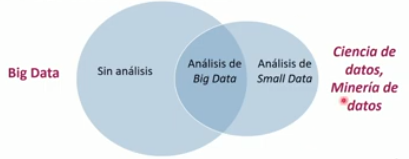
\includegraphics[scale=0.95]{images/mod01-01.png}
\end{center}

\begin{itemize}
    \item Podemos tener un conjunto de datos pequeños, por ejemplo, pruebas diagnósticas de un número reducido de pacientes, y analizar esa información. Formaría parte del \ti{Análisis de Small Data}.
    \item Podemos tener millones de registros de pacientes con medicamentos y tratamientos, de los que queremos analizar esos datos, hablaríamos de \ti{Análisis de Big Data}.
    \item Por último, podemos tener los datos de todas las compras que se han realizado en un país durante unos cuantos meses o años y visualizar esos datos o resumirlos o hacer un informe y tener una gran complejidad a la hora de integrar esos datos o transformalos, pero sin un análisis, hablariamos de \ti{Big Data}.
\end{itemize}

Es importante ver una serie de términos que están relacionados cuando hablamos de ciencia de datos y el papel del machine learning junto a la ciencia de datos.

\begin{center}
    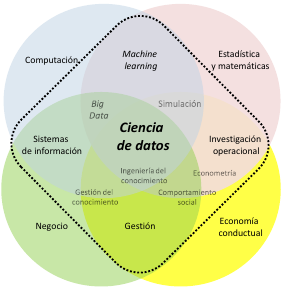
\includegraphics[scale=0.95]{images/mod01-02.png}
\end{center}

\section{Minería de Datos y Ciencia de Datos}

Para entender lo que es la \ti{ciencia de datos}, centrándonos particularmente en la \ti{minería de datos}, la transformación de datos a conocimientos, vamos a ver cuatro ejemplos:
\begin{itemize}
    \item Agente bancario. ¿Debo ofrecerle una hipoteca al cliente?. Veremos que con determinadas herramientas, que extraen conocimiento, modelos  a partir de datos podremos resolver la pregunta.
    \item Gerente de supermercado. ¿Cuando los clientes compran huevos, también comprarán aceites?. Aquí veremos que podemos utilizar herramientas, de minería de datos, no tanto de análisis descriptivo o de aprendizaje automático.
    \item Gerente de personal. ¿Qué tipo de empleados tengo?.
    \item Supervisor de fábrica. ¿Cuántos fallos, para el módulo \ti{X} esperamos cada mes?, o ¿Cuántas ventas vamos ha hacer?.
\end{itemize}

\subsection{Agente bancario}

Cuando un cliente solicita una hipoteca o un préstamo de autoconsumo, la respuesta debe ser si se le concede o no. Para responder a esta situación, lo que le interesa al banco es saber si \ti{los clientes anteriores han sido buenos clientes o malos para el banco}.

\begin{center}
    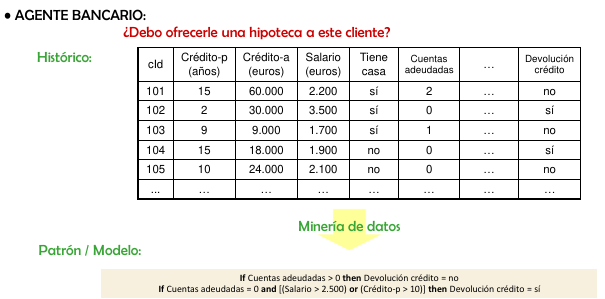
\includegraphics[scale=.8]{images/mod01-03.png}
\end{center}

Un cliente que no devuelve un crédito es un \ti{mal cliente para el banco}, pero puede haber otros conocimientos, como por ejemplo, un mes no se paga la mensualidad, no es un problema muy grande si después el cliente se recupera y puede ser incluso beneficioso para el banco. Lo que debe tener registrado el banco no es sólo si se devolvió o no el crédito, sino si realmente ha sido beneficioso o no para el banco.

Sit tuviéramos miles y miles de clientes anteriores a los que hemos concedido un préstamo, podríamos saber si al final, y al cabo de un cierto tiempo, esa persona ha tendio problemas o no a la hora de devolver el crédito.

Cuando un cliente solicita un crédito suelen hacérsele una serie de preguntas: cuanto tiempo durará el crédito, cuanta cantidad se solicita, que ingresos mensuales tiene, así como otro tipo de preguntas sobre su entorno familiar o si tiene otro tipo de propiedades que puedieran utilizarse como aval . La table mostrada está bastante simplificada, en relación al tipo de preguntas que se pueden realizar.

Toda esta información se registra en una base de datos relacional. Ahora recibimos un nuevo cliente, que nos pide unos años, nos indica el dinero que quiere pedir y le hacemos otra serie de preguntas, lo que no sabemos es qué le responderemos. ¿Cómo podemos responder a esta petición?. Para ello lo que haremos será transformar los datos de la tabla en un modelo que a partir de las entradas del nuevo cliente nos de la predicción de si debemos conceder o no el crédito.

En este caso estamos realizando una \tb{tarea predictiva}, y en este caso de \tb{clasificación}, donde los datos de entrada se corresponden con las conlumnas de la tabla, salvo la última columna, \ti{«devolución crédito»}, que se corresponde con nuestra variable de salida o predicción.

Como ejemplo, el modelo nos indica las siguientes reglas:
\begin{itemize}
    \item que si \ti{las cuentas adeudar son mayores que cero, entonces, no devolverá el crédito}
    \item \ti{si las cuentas adeudadas son igual a cero y el salario es mayor de 2.500€ o los años son mayores que diez, entonces, normalmente se devuelve el crédito}.
\end{itemize}

Se trataría de un modelo muy simplista, pero nos da una solución al problema.

\subsection{Gerente supermecado}


Es un caso muy general en el ámbito del análisis de datos, puede ocurrir en cualquier tienda online o cualquier medio por el que se compran productos conjuntamente.

\begin{center}
    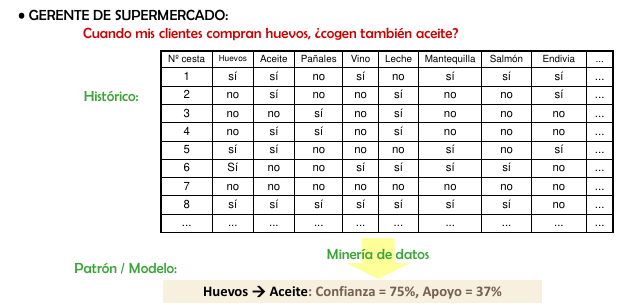
\includegraphics[scale=.8]{images/mod01-04.png}
\end{center}

Uno puede preguntarse, ¿Qué productos se compran conjuntamente? o cuando uno sale con la cesta, qué suele acompañar a éstos productos. En principio, si son pocos productos, se puede observar directamente, pero si son muchísimos productos, como un supermercado que puede tener miles de productos en su stock, si queremos ver que productos se compran conjuntamente, se pueden buscar todas las compras hechas durante y una semana, que previamente se ha registrado en una tabla como la de la imagen, y comprobar si los \ti{«síes»} de una columna están asociados con los \ti{«síes»} de la otra columna.

En la table vemos que aceites y pañales no estarían demasiado asociados.

Lo que queremos es responder a la pregunta general ¿qué productos se compran conjuntamente? Esto nos obliga a ver todas las combinaciones posibles de pares entre los miles de productos; para ello podemos recurrir a \ti{herramientas de minería de datos} que lo que hacen es extraer todas las asociaciones, relaciones entre atributos que son muy frecuentes.

Cuando ejecutamos el análisis de datos, en relación con la pregunta \ti{"cuando los clientes compran huevos, ¿compran también aceite?"}, obtendremos un patrón que dice que cuando se compran huevos, entonces se compra aceite y la confianza es un 75\%, quiere decir que de 100 compras de huevos, en 75 ocasiones también se compra aceite. Aún así, puede que ambos productos estén muy relacionados pero sean poco frecuentes en conjunto.

En el caso visto, los atributos de la tabla son todos de entrada, no hay variables de salida, en este caso hemos obtenido un modelo que establece una regla o patrón que nos indica la relación entre dos productos.

\subsection{Gerente de personal}


En este caso, un gerente de personal se pregunta \ti{¿qué empleados tengo?}. De los empleados a su cargo conoce algunos, pero dependendiendo del número de empleados de la empresa es probable que desconozca a la gran mayoría. Necesito información, datos, para tomar decisiones respecto a la restructuración de la empresa, si tengo que formarlos de alguna manera o cualquier otra actividad que les afecte.

\begin{center}
    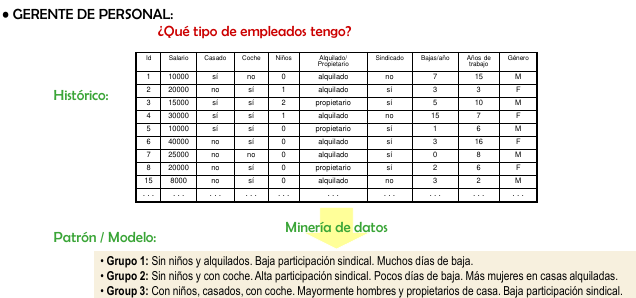
\includegraphics[scale=.8]{images/mod01-05.png}
\end{center}

Toda empresa suele tener una base de datos con la información importante relacionada con sus empleados, como puede ser: el salario, si tiene coche, si está casado, \ldots A partir de esa información, quiero poder conocer \tb{qué tiplogías o grupos de empleados tiene la empresa}.

A simple vista podríamos tener una idea general, pero la gradación que puede haber de unos empleados a otros, teniendo atributos similares, es tanta que nos perderíamos y no concretaríamos dichas tipologías. Para ayudarnos hay herramientas de \tb{aprendizaje automático, de agrupamiento, de clustering} que nos permitirán, a partir de los datos de la tabla, todos los atributos son de entrada, desarrollan un algoritmo que nos generará tres grupos, los cuales agrupan registros que se parecen y difieren de los registros de otros grupos.

En el ejemplo vemos que los tres grupos se componen:
\begin{itemize}
    \item \tb{Grupo 1}: sin hijos, con vivienda en alquiler, baja participación sindical y con muchos días de baja.
    \item \tb{Grupo 2}: sin hijos, que tienen coche, alta participación sindical, pocos días de baja y más mujeres que hombres en casas alquidas.
    \item \tb{Grupo 3}: con hijos, casados, con coche, mayoritariamente hombre y con vivienda en propiedad, baja participación sindical.
\end{itemize}

La herramienta crea los grupos, en función de nuestras necesidades.

\subsection{Supervisor de fábrica}

Aquí puede interesarnos contestar a la pregunta \ti{¿Cuántos fallos para el módulo «X» esperamos cada mes?}. Disponemos de una serie de datos relativos a ese módulo, entre ellos como ha ido fallando.

\begin{center}
    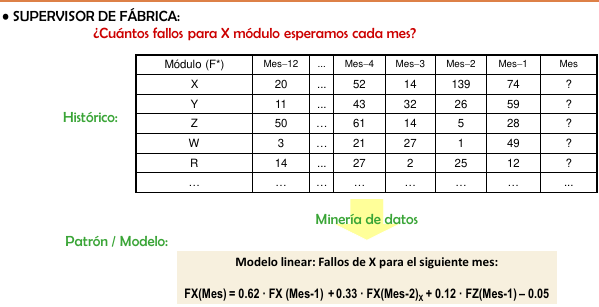
\includegraphics[scale=.8]{images/mod01-06.png}
\end{center}

Se trata de un problema más complejo que los anteriores ya que involucra el \ti{tiempo}, los otros ejemplos vistos no son atemporales, pero en éste tendremos información relativa a los fallos que cada módulo ha podido tener cada mes.

Muchas veces las predicciones, sobre todo relativas al tiempo, se bansan en los valores, no sólo del tiempo inmediatamente anterior, sino de valores agregados en tiempos o en ciclos anuales, mensuales, \ldots A partir de aquí, con el procesameinto de los datos, indicándole qué queremos predecir, los fallos para el mes que viene, partimos de la información sobre fallos de los meses anteriores, información que puede depender del propio módulo, pero también de fallos de otros módulos, con lo que la información que podemos incluir para predecir el valor de \ti{X}, puede depender de sus valores, pero también de la información de otros registros del resto de módulos.

En este caso, utilizando la tabla referida y mediante una herramienta de minería de datos, con una preparación concreta, procesarimos los atributos necesarios como entradas, para obtener la última columna que se corresponde con la salida tras el procesamiento.

En este caso, podríamos utilizar una función lineal como la que se indica a continuación, en concreto \ti{regresión lineal}, que predice un valor numérico, los fallos de el módulo \ti{X}:
$$FX(Mes) = 0.62\ast FX(Mes_1) + 0.33\ast FX(Mes_2) + 0.12\ast FZ(Mes_1) - 0.05$$

\begin{itemize}
    \item $Mes_1$, mes anterior al que queremos predecir.
    \item $Mes_2$, dos meses antes.
    \item $FX$ referido a los fallos de otros módulos.
    \item Los coeficientes: 0.62, 0.33, 0.12 y 0.05, son proporciondos por la herramienta de minería utilizad.
\end{itemize}

El modelo es \tb{predictivo}, pero en este caso es un \tb{modelo de regresión}.

\subsection{Papel de la inteligencia empresarial}

\tb{Inteligencia Empresarial} es un concepto que engloba una serie de herramientas que intenta extaer conocimiento y tomar decisiones a partir de la información. Son herramientas que se estructuran en varios niveles, se conoce como estructura piramidal, desde los datos más básicos hasta el conocimiento.

\begin{center}
    \begin{tabular}{ c c }
        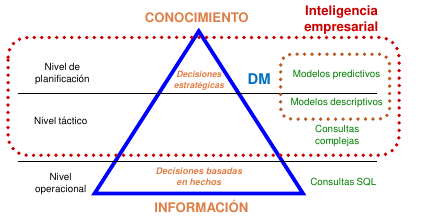
\includegraphics[scale=.8]{images/mod01-07.png} &
        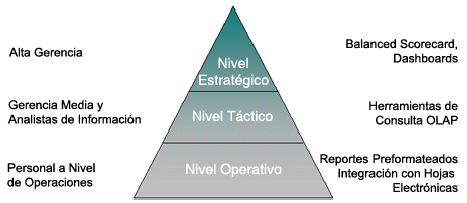
\includegraphics[scale=.5]{images/mod01-07_1.png}
    \end{tabular}
    
\end{center}

Un ejemplo sencillo sería que \ti{quiero reservar un vuelo desde Valencia a Montevideo, con varias escalas}, lo que haré será mirar a través de una aplicación, que me solicitará el origen, el destino, los días, etc; esta aplicación lo que hará es localizar los vuelos que tiene en su base de datos que coincidan con los datos aportados y si hay espacio en ellos proporniendolos como rutas posibles. Una vez que quiero realizar la transacción, la reserva, la aplicación deberá comprobar en todo momento que sigue habiendo plazas disponibles, y finalizada la transacción, si había plaza, confirmar la transacción.

La decisión que toma el sistema \tb{no es estratégica} es una decisión a nivel \tb{operacional}, que los sistemas pueden tomar en todo momento basándose en información, que normalmente se recoge en bases de datos, que internamente se consultan y modifican a través de lenguajes de gestión de bases de datos, como SQL. 

Todo el proceso visto constituiria la base de la piramide, la interacciones más sencillas entre un dispositivo o aplicación y una persona.

Por encima del \tb{nivel operacional} hablaríamos del \tb{nivel táctico}, en él podemos hacer consultas mucho más complejas, como el informe que llega a la mesa de algunas personas, que toman decisiones en la organización, como pueden ser las ventas de la última semana, mes o año, desglosados por zonas geográficas y por tipos de productos. Son informes que van más allá de lo que es el dato preciso o concreto, no es información hipotética, sino de hechos ocurridos y, a partir de los cuales, tomar decisiones. Esta información se puede obtener a partir de consultas complejas, mediante instrucciones de lenguaje de programación como \ti{group by}, agrupamiento, información que suele acompañarse de gráficos.

La información obtenida a nivel táctico podemos transformarla en \tb{conocimiento} y observar si las ventas han ido como queríamos o si hay algo sorporendente.

El \tb{nivel de planificación}, está por encima del nivel táctico, e incluye decisiones más complejas, por ejemplo decidir si \ti{tengo que hacer una oferta a un clinte o conceder un crédito a un usuario}, no son preguntas que se puedan obtener de forma directa de los registros de una base de datos, ya que lo que necesitamos es anticipar o entender el conjunto de datos, de que disponemos, entender el histórico y, a partir de ahí, extrapolar (puede ser desde el punto de vista predictivo o de grupos o tipologías). Este tipo de decisiones a este nivel, si queremos automatizarlas, requieren de herramientas de \ti{aprendizaje automático}, la minería de datos nos permite tener modelos descritivos o predictivos que nos permitan tomar decisiones.

Vemos que a medida que ascendemos en la pirámide se requieren herramientas cada vez más sofisticadas.

La \ti{inteligencia empresarial} es un térino que engloba las herramientas de tecnología de la información y normalmente suelen estar compuesta de tres áreas:

\begin{itemize}
    \item herramientas de almacenamiento de datos y OLAP, permiten manejar volumnes de información y combinarlos, agregarlos y rotarlos.
    \item paneles de control y herramientas de supervisión, permiten a través de gráficas ver como va la organización en todo momento o unirlos a los informes.
    \item herramientas de minería de datos, permiten extaer de estos datos modelos con los que tomar decisiones; son modelos que pueden ser predictivos o descriptivos.
\end{itemize}

\subsection{Minería de datos}

Una estructura básica, sin entrar en detalles, de como se organiza la \ti{inteligencia empresarial} sería la representada en el gráfico.

\begin{center}
    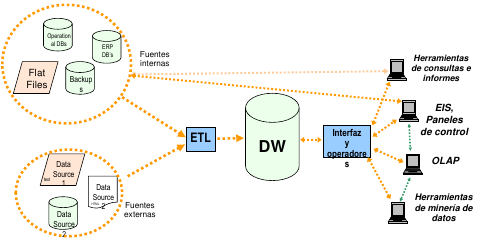
\includegraphics[scale=.8]{images/mod01-08.png}
\end{center}

En primer lugar, al analizar datos e integrarlos para tomar decisiones estratégicas utilizaremos tanto las fuentes internas de la organización como las externas. Fuentes internas suelen ser el sistema de información de la organización, información que se vuelca en un \ti{almacén de datos}, que generalmente está desconectado del trabajo diario de la organización. Normalmente, la fuentes internas, no permiten una visión completa del entorno de la organización, en la organización funciona normalmente un entorno económico y social y se requieren datos e información del exterior, como pueden ser: tendencias del sector, qué eventos están ocurriendo. Temas como meteorología y calendarios, son fundamentales a la hora de hacer modelos predictivos; es información que podríamos necesitar integrarla, no es información necesaria desde el punto de vista operacional o trasaccional, pero es fundamental a la hora de extraer modelos que sean realmente predictivos y descriptivos sobre lo que ocurre alrededor de la organización. 

Es una información, que como externa, puede estar en muchas fuentes diferentes, en bases de datos que uno compra o que están disponibles gratuitamente, de informes textuales, muchas veces en páginas web, \ldots

Como hemos dicho todo se integra en una base de datos o almacén de datos, que podemos ver que podemos organizarlos de diferentes maneras y, sobre esta información integrada, podemos aplicar una serie de herramientas con las que extraer informes.

Por último, tenemos \ti{paneles de control} y \ti{sistemas de información ejecutivos} que pueden hacer lo mismo. Las herramientas \ti{OLAP} son herramientas que permiten, una vez realizada una consulta compleja que incluye la selección de varias dimensiones de los datos y agregadas a distintos niveles, entre otras:
\begin{itemize}
    \item cambiar rápidamente entre niveles
    \item avanzar la consulta sin tener que esperar a que ésta acabe
\end{itemize} 

Las herramientas de minería de datos permiten a través de los datos históricos generar vistas \ti{minables} y extraer modelos descriptivos y predictivos a partir de estas vistas.

\subsection{Almacenamiento de datos multidimensional}

Los alamacenes de datos normalmente se organizan como una base de datos, integrando información de diferentes fuentes que posean información valiosa desde el punto de vista de responder a cuestiones de tipo estratégico, más que de tipo transaccional.

\begin{center}
    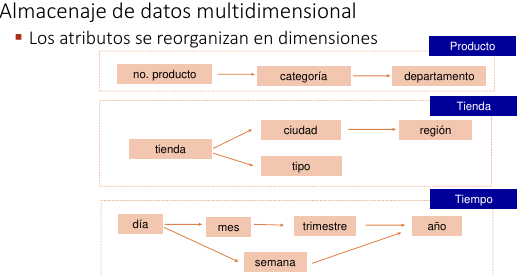
\includegraphics[scale=.8]{images/mod01-09.png}
\end{center}

Para el trabajo transaccional utilizamos la base de datos de toda la vida, generalmente relacional.

Cuando el almacén de datos es sólo para realizar consultas, no habrá actualizaciones ya que estas normalmente van a la base de datos transaccional, ¿qué tipo de organización es más habitual?. Desde el punto de vista de la organización del almacén de datos tenemos, lo que se conoce como \tb{modelo multidimensional}, es un modelo muy intuitivo ya que la información se suele dividir en dimensiones, que nos permiten agregar o desagregar la información a través de esas dimensiones.

Tomemos el ejemplo de un supermercado. En un supermercado puedo realizar las típicas preguntas o adverbios interrogativos:
\begin{itemize}
    \item ¿Qué es lo que se vende en el supermercado?, hablamos del producto.
    \item ¿Dónde se vende?, nos aparece la dimensión tienda.
    \item ¿Cuándo se vendió?, nos aparece la dimensión temporal, cada producto se ha vendido en una tienda en un momento determinado.
\end{itemize}

Podemos hacer más preguntas como el tipo de pago, la hora, etc.

Nos vamos a centrar en qué, dónde y cuándo.

\begin{itemize}
    \item El \tb{qué}, hablamos del producto, cuando intentamos analizarlos vemos que se organizan jerárquicamente o en diferentes niveles. En general, del producto tenemos la siguiente información:
    \begin{itemize}
        \item número del producto o código.
        \item categorias.
        \item departamentos.
    \end{itemize}
    Puede haber más subdivisiones, aunque por simplicidad sólo mostramos tres.
    \item El \tb{dónde}, referencia al punto de venta, una tienda concreta o venta online. En una tienda podríamos subdividir, incluso, por cajas. Podrían agregarse el tipo de tienda: minis, grandes o grandes superficies, \ldots Podemos agregar una dimensión \ti{geográfica}: ciudad, región, país, \ldots
    \item El \tb{cuándo}, el tiempo o momento en que se realizó la venta, bien el día, semana, mes, año, etc, incluso añadir más nivel de granularidad como la hora y minuto.
\end{itemize}

Este tipo de dimensiones y jerarquías de los niveles es parte del \ti{diseño multidimensional} de este tipo de almacén de datos.

¿Cómo funcionan?. Hablabamos de ventas, para este caso sería la información que tendremos sobre prductos, lugar y tiempo. 

\begin{center}
    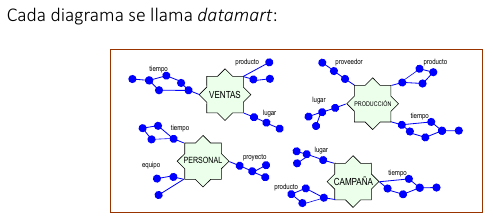
\includegraphics[scale=.8]{images/mod01-10.png}
\end{center}

Podríamos tener otros subalmacenes que normalmente se concocen con el nombre de \tb{datamarts} en el que la información es de otro tipo. Para producción, podríamos tener información sobre campañas, que podrían ser independientes de la información de ventas. Cada una de ellas sería un \ti{datamart} y cada uno de éstos tiene su estructura multidimensional.

Analicemos el \ti{datamart de ventas}. Tenemos un ejemplo de una consulta, de momento ignoramos la parte de OLAP. 

\begin{center}
    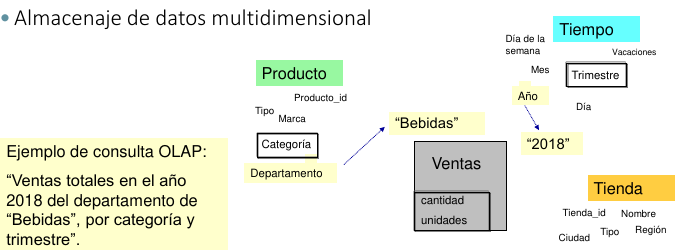
\includegraphics[scale=.8]{images/mod01-11.png}
\end{center}

Quiero saber las ventas totales en el año 2018, del departamento de bebidas, por categorías y por trimestre.

\begin{enumerate}
    \item Nos centramos en el \ti{datamart de ventas}, encontramos que hay una tabla central que tiene la información de los indicadores, en este caso cantidad(precio) y unidades. 
    \item Como cualquier pregunta suelen estar asociados con el qué, cuándo y cómo. En nuestro caso, el indicador son las ventas en el año 2018, tendremos que irnos al tiempo, en esta diménsión agregará \ti{año}, en la dimensión de productos agregará la dimensión \ti{departamento},\ti{bebidas}.
    \item Por último, categoría y trimestre. Estos atributos no son selecciones sino agrupamientos.
\end{enumerate}

Obtendriamos una tabla con la información seleccionada. Esto nos da un resultado que puede representarse de esta forma:

\begin{center}
    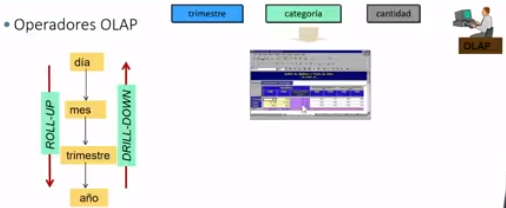
\includegraphics[scale=.8]{images/mod01-12.png}
\end{center}

Podríamos ponerlo como una tabla en el que las categorías son las filas y los trimestres las columnas, y cada celda, las ventas totales.

Ahora podríamos querer cambiar algo en la consulta, para ello utilizarmos las \ti{herramientas OLAP (OnLine Analitic Processing o Proceso analítico online)} para realizar un refinamiento de las consultas sin tener que lanzar una nueva consulta. En nuestro caso podríamos hacer, lo que se conoce com \ti{drill down}, ir de trimestre a mes sin tener que realizar un informe nuevo, sino desde el informe original.

\begin{center}
    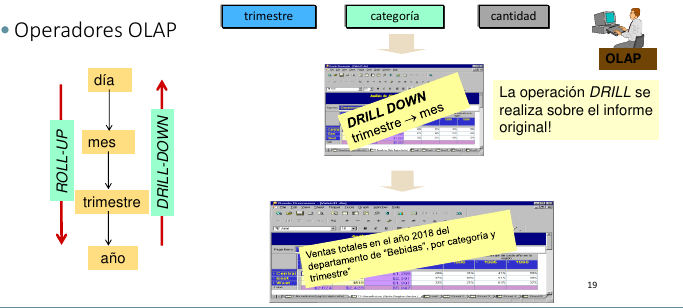
\includegraphics[scale=.8]{images/mod01-12_1.png}
\end{center}

\subsection{OLAP vs Minería de Datos}

¿Es \tb{OLAP} lo mismo que aprendizaje automático, que la minería de datos?. En principio, son cosas diferentes, aunque existe una delgada línea entre las preguntas que pueden responderse con herramientas de minería de datos o técnicas de aprendizaje automático y las que se pueden responder con herramientas \ti{OLAP}, un almacén de datos y sin extrapolar.

La línea que separaría ambos ámbitos, es que \ti{OLAP}, aunque sea de manera agregada, de manera compleja, todo el tipo de consultas estratégicas que hacemos sobre el almacén de datos no dejan de ser consultas sobre datos que existen en dicho almacén, la consulta no se inventa nada, no hace ninguna extrapolación ni hipótesis sobre los datos. Sin embargo, cuando hablamos de \ti{minería de datos}, aquí existe un razonamiento hipotético, normalmente inductivo. 

En la tabla tenemos preguntas que podemos clasificar en un de los dos ámbitos vistos.

\begin{center}
    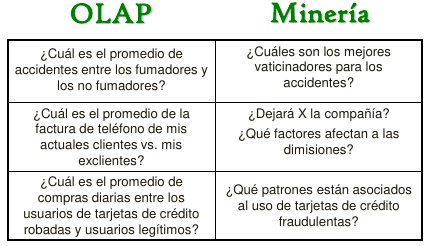
\includegraphics[scale=.8]{images/mod01-13.png}
\end{center}

Las preguntas que aparecen en la columna de \ti{OLAP} vemos que son datos que se encuentran en el almacén de datos, y que lo que hacemos es lanzar consultas sobre datos reales recogidos en ellas, sin tener que elaborarlos. Por el contrario, en el lado de la \ti{minería}, la información tienen que se interpretada, requiere la elaboración de un \ti{modelo hipotético} que relacione las entradas, en el caso de la primera pregunta, las características de los clientes como: edad, sexo, años de antiguedad del carnet, tipo de comportamiento, dónde vive y demás, con respecto al número de accidentes que pueda tener; esto se hace a través de información histórica y no de información futura, que nos permite entender cuál es esta relación y describe lo ocurrido de forma abstracta.

En relación con la pregunta ¿qué patrones están asociados al uso de tarjetas de crédito fraudulentas?, la pregunta es bastante más amplia, aquí lo que podemos responder son cuestiones que son anómalas, por ejemplo, realizar dos o más compras de un tipo concreto, puede estar asociado a un uso fraudulento de las tarjetas, ya que normalmente son compras, por ejemplo, en joyería, alguien que nunca ha comprado este tipo de artículos y por cantidades elevadas, son pagos bastante inusuales para el perfíl del individuo; aquí se recurriría a herramientas de aprendizaje automático principalmente, para extraer ese tipo de patrones.

De las siguientes afirmación, cuales pueden resolverese mediante herramientas \tb{OLAP}:

\begin{enumerate}[label=\Alph*)]
    \item ¿Cuál es el producto más vendido entre el rango de edad 25-45?
    \item ¿Cuántos productos de la categoría «hogar» se espera vender el año que viene?
    \item ¿Qué diferencia de tamaño hay entre las cestas de la compra de los sábados y entre semana?
    \item ¿Qué días del mes suele haber más rotura de stock?
    \item ¿Qué tipo de productos tengo atendiendo a sus características: peso, precio, etc.?
\end{enumerate}

Las respuestas correctas son \ti{A),C) y D)}.

\subsection{Ejemplos de Ciencia de Datos}

La \ti{ciencia de datos} en un contexto de \ti{inteligencia de negocio} es una actitud más que una disciplina desde el punto de vista de una organización. Cuando una organización contrata un científico de datos, lo que quiere es una persona con un rol muy particular.

Podemos pensar que un científico de datos es lo mismo que otros roles existentes en las organizaciones: director de sistemas de información o \ti{data manager} o el director de datos o \ti{data officier}. En empresas relacionadas con la tecnología, son roles muy importantes en la organización, son roles de primer nivel, como el caso de Google o Fracebook, donde lo más importante son los datos. El científico de datos va en esa línea, debería ser una persona con un conjunto integrado de habilidades que abarcan:
\begin{itemize}
    \item matemáticas
    \item aprendizaje automático
    \item inteligencia artificial
    \item estadística
    \item optimización de bases de datos
\end{itemize}
pero con un profundo conocimiento en la elaboración de problemas para el diseño de soluciones efectivas. Su función debe ser extaer valor de los datos y sacar valor a partir de ellos, haciendo que éstos sean el motor de la organización, no simplemente una herramienta que existe en la organización  que está ahí para el funcionamiento de las aplicaciones, sino conseguir que esos datos sean los que proporcione valor y hagan que la organización funcione.


Nos podemos preguntar ¿dónde se originan esos datos? y ¿para quién queremos obtener ese valor?. Dependendiendo de estas preguntas podemos clasificar distintos tipos de aplicaciones o problemas que podemos resolver mediante la ciencia de datos.

\begin{itemize}
    \item Los datos que tengo son valiosos para mí ($in\,\rightarrow\,in$), prácticamente el 100\% de las organizaciones que tengan datos pueden sacar rendimiento a partir de ellos, a parte de lo que pueda ser el sistema transaccional, pueden sacar valor, sacar patrones que ayuden a la hora de la toma de decisiones. Aunque hablamos de organizaciones es extensible a los individuos. Esto es lo que se ha conocido como \ti{inteligencia empresarial clásica}.
    
    Cuando hablamos de \tb{datos internos de la organización} para dar servicio a la orgnización, un ejemplo habitual es el de una compañía de seguros de automóviles donde queremos predecir qué póliza va a comprar un cliente. Teniendo en cuenta su historial de transacciones, miro el almacén de datos y extraigo los datos que me permitan establecer un \ti{modelo predictivo} sobre qué póliza es la más adecuada. No necesita buscar datos fuera de la organización.

    \item Los datos que he visto exteriores a la organización, los podría utilizar para sacar patrones que me ayuden en mis decisiones ($out\,\rightarrow\,in$), dichas fuentes pueden ser redes sociales.
    
    Como ejemplo, tenemos la \ti{Comisión del Crimen de Detroit}, en su momento intentaron utilizar información sobre redes sociales para ver realmente dónde y en qué momentos se estaba produciendo tráfico de drogas u otro tipo de delincuncia. Es sorprendente, pero algunos delincuentes son capaces de decir lo que están haciendo en las redes sociales o de lo que van a hacer o dónde van a quedar, a partir de ahí la policía puede saber qué puntos calientes hay, e incluso poder abortar algunos de los posibles delitos. Son datos completamente externos que le permiten tomar decisiones estratégicas.

    \item Nosotros disponemos de datos, que son valiosos para nosotros, pero también podrían serlo para otras organizaciones externas ($in\,\rightarrow\,out$), como sacar esos datos es un servicio que los pone disponibles. Podemos vender los datos directamente o el «conocimiento», como se extrae dicho conocimiento.
    
    Cuando hablamos de externos, por ejemplo una compañía de telefonía, sus clientes no son externos son internos, al hablar de externos nos referimos que somos conscientes de que tengo información sobre miles de usuarios, que son internos, y que es información puede ser útil para terceros. Por ejemplo, tendría información de dónde se encuentran los usuarios en una ciudad, si tengo el 20\% de cuota de teléfonos móviles en una localidad, puedo saber dónde están, no a nivel individual, esta información no se puede proporcionar a terceros por razones legales, pero sí a nivel \ti{agregado}. Puedo saber que proporción de gente se mueve en una zona de la ciudad en un rango de horas. Si mi porcentaje es lo suficientemente representativo, podré extrapolar y saber los flujos de población en la ciudad. Esta información puede ser importante para ayuntamientos, comercios, transportes, etc. Evidentemente, el poseedor de la información sacará un beneficio de proporcionar este conocimiento.

    \item En ocasiones, yo no tengo los datos, ni siquiera soy el fin, soy un intermediario ($out\,\rightarrow\,out$), un experto en ciencia de datos que dispone de los datos y establece que si se extrajeran determinados patrones, los datos podrían ser útiles para una organización o usuarios. Muchos servicios hoy en día intentan hacer este tipo de cosas.
    
    Cómo en casos anteriores, recurrimos a las redes sociales. La gente, con frecuencia, cuando se encuentran mal, enfermos, pueden indicar sus síntomas e incluso que acudieron al médico e indicar que pronóstico les dió en redes sociales. Se intenta hacer asociaciones entre síntomas, como se toman los medicamentos, etc. Es una información que es externa, y que estaba dirigida para otro tipo de uso.

    \item Finalmente, la visión más ambiciosa, no hay datos ($\emptyset\,\rightarrow\,out$), pero si los hubiera habría valor, es decir puedo intentar crear aplicaciones cuyo objetivo final sea crear datos que den valor. Gran parte de la economía digital reciente se basa en esta idea. Si volvemos a las redes sociales, éstas a partir de la nada han creado datos, a partir de éstos conocen el perfíl de la gente, sus aficiones, gustus, horas de contacto, amigos, familiares, es decir, no es que esa información existiera, pero mucha se crea a través de esas aplicaciones que se crean inicialmente de la nada.
    
    Una de las aplicaciones más típicas, relacionadas con este punto de vista, es que instalamos una aplicación en nuestro dispositivo móvil que nos informa, a través de datos que recoge de otros usuarios de la misma aplicación. El ejemplo típico son aplicaciones de tráfico, nos permiten saber las rutas más cortas y menos congestionadas.
\end{itemize}

Otra forma de ver la ciencia de datos es en las áreas donde se aplica, aquí podemos ver algunas de ellas:

\begin{center}
    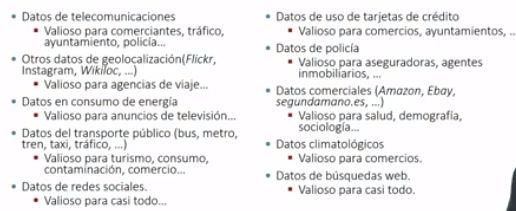
\includegraphics[scale=.9]{images/mod01-14.png}
\end{center}

\section{Proceso de extracción de conocimiento}

Cuando nos centramos en la parte de la \ti{minería de datos}, más predictiva o descriptiva, nos centramos en convertir datos en conocimiento, proceso que se conoce por sus siglas en inglés de \tb{D2K (Data to Knowledge)}, de datos a conocimiento.

\begin{center}
    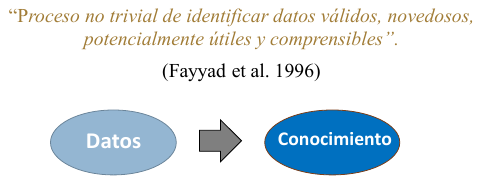
\includegraphics[scale=.9]{images/mod01-15.png}
\end{center}

Este proceso podemos traducirlo como extracción de conocimiento a partir de datos o bases de datos de cualquier tipo. Es un proceso que se conoce hace tiempo, no trivial de identificar patrones válidos, potencialmente útiles y comprensibles.

\begin{itemize}
    \item Es un \tb{proceso no trivial}, si fuera sencillo no serían necesarias herramientas, de conocimiento o relgas o técnicas para resolver el problema.
    \item \tb{Identificar patrones}, son patrones que van más allaá de los datos, son tendencias, reglas, grupos que no son sólo datos agregados; normalmente infieren otro tipo de información a partir de los datos ya existentes. Como son datos hipotéticos, que extrapolan a partir de otros datos, históricos, nos interesa que sean válidos, que los patrones tengan un porcentaje de error mínimo. La parte de evaluación es fundamental.
    \item \tb{Novedoso}, por ejemplo que en una unidad de maternidad de un hospital, el porcentaje de ingresos de mujeres siempre será del 100\%, este procedimiento no es novedoso. También se da el caso de ser novedoso pero inútil, puedo suponer que dos productos, champú y una marca de tomate se compran conjuntamente, ¿qué puedo hacer con esa información?, poner el champú cerca del tomate, probablemente será una curiosidad, pero difícilmente será útil.
    \item La información debe de ser \tb{comprensible}, hablamos de técnicas de aprendizaje automático, redes neuronales o redes profundas, máquinas de vectores, que proporcionan información poco comprensible para un humano, frente a técnicas que producen reglas que sí son comprensibles por un humano, como pueden ser los árboles de decisión.
\end{itemize}

Este proceso normalmente se desglosa en fases más concretas, no sólo en cómo convertir datos en conocimiento

\begin{center}
    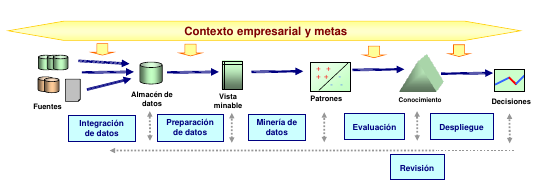
\includegraphics[scale=.9]{images/mod01-16.png}
\end{center}
en la parte izquierda tenemos el conocimiento, el final aparace como decisiones, apartir de ese conocimiento, es lo que se denomina extracción del conocimiento a partir de datos.

El número de tareas o de fases puede variar, pero generalmente se empieza por una parte de integración de datos, con fuentes internas y externas con distintos formatos, que integraremos generalmente en un repositorio, que no tiene por qué ser multidimensional, pero sí un repositorio donde tenemos todos los datos juntos, integrados y consistentes. Aunque tengamos todo los datos almacenados, será necesario prepararlos para el modelo que queremos extraer. Este proceso de preparar para extaer conocimiento es lo que se conoce como \ti{crear la vista minable}.

En la vista minable pongo una filas y columnas con la información que quiero, una vez que tengo todo esto puedo aplicar minería de datos, o aprendizaje automático, para obtener patrones, que normalmente tendré que evaluar, tendrán un error, fallarán con alguno de los ejemplos del histórico. Habrá que seleccionar aquel patrón que mejor se ajuste a los datos y que tenga un menor error.

Una vez realizado el proceso, dispondremos de un \tb{modelo evaluado y validado}, y hablamos realmente de conocimiento, ya podremos utilizarlos y tomar decisiones.

Estos modelos en ocasiones quedarán obsoletos, las situaciones cambian o aparecen problemas inesperados; podemos ir hacia atrás, al inicio o a un reentrenamiento de los modelos dependiendo del problema que detectemos.


\subsection{Estándar CRISP-DM}

Hemos visto que el proceso de extración de conocimiento se estructura en una serie de fases, que pueden variar dependiendo del contexto o de la organización, incluso podemos ver el proceso a partir de conocimiento muy simple. 

Cuando vemos un proceso que tiene que seguir una serie de pasos aparecen estándares o metodologías que guían el proceso. Seguir estos estándares permite que diferentes usuarios, e incluso organizaciones, se entiendan a la hora de desarrollar un proyecto. Un proyecto ya finalizado, es más entendible si sigue una metodología.

Algo importante de las metodologías es que van acompañadas de documentación, que permite que los usuarios externos al proyecto puedan entender e integrarse en el proyecto más fácilmente. No es más que \tb{gestión de proyectos} aplicado a ciencia de datos.

La metodología más común se conoce como \tb{CRISP-DM}, apareció hace más de veinte años, como un proyecto de la comisión europea y de empresas, siendo una de las metodologías más utilizadas.

La metodología CRISP-DM se conceptualiza en 6 fases:

\begin{center}
    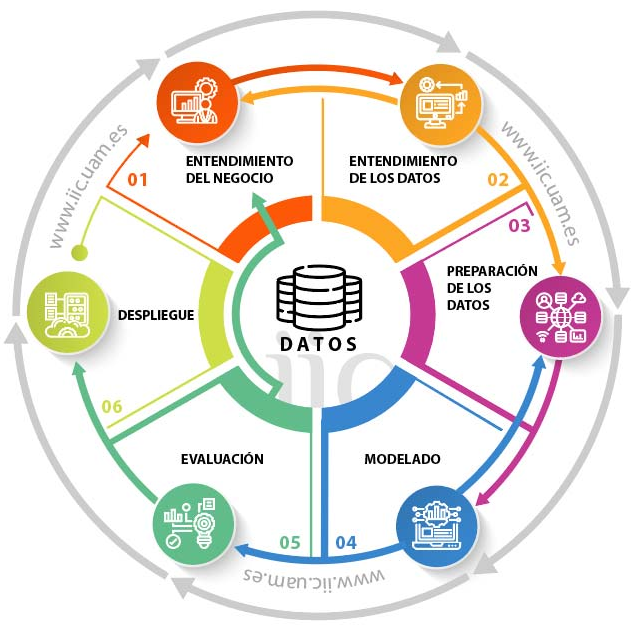
\includegraphics[scale=.6]{images/mod01-17.png}
\end{center}

\begin{enumerate}
    \item \tb{Entendimiento del negocio}, el equipo de trabajo debe comprender los objetivos y requisitos del proyecto definidos por el cliente, para convertir el conocimiento en una definición técnica del problema. Require una comunicación intensa entre cliente y equipo técnico.
    \item \tb{Entendimiento o compresión de los datos}, el equipo técnico realiza un \ti{análisis exploratorio} para obtener una visión general de lo que se puede conseguir con los datos. Tras el análisis debiería tenerse una idea clara de la viabilidad del proyecto y de los resultados esperados, de ser así se avanza a las siguientes dos fase.
    \item \tb{Preparación de los datos}, cubre las actividades para construir el conjunto de datos definitivo que se empleará en la siguiente fase.
    \item \tb{Modelado de datos}, el equipo técnico realiza los análsis y modelos pertinentes de los que se deriven los resultados y conclusiones del proyecto, y su validación frente a errores.
    \item \tb{Evaluación}, el cliente determinará la calidad de los resultados obtenidos y decidirá cómo pueden explotarse antes del despliegue.
    \item \tb{Despliegue}, fase en la que el modelo se pone en producción, con el fin de tomar decisiones.
\end{enumerate}

Se trata de un proceso de \tb{carácter iterativo}. Aunque algunos consideran que esta metodología es un poco rígida, siempre puede ser utilizada como base y adaptarla a nuestras necesidades.

\section{Tareas, técnicas y herramientas}

\subsection{Tareas}

Algo muy importante es distinguir entre tareas, técnicas y herramientas. Nos vamos a centrar ahora en ¿qué son las tareas?.

Vamos a ver cinco grandes familias de tareas:
\begin{itemize}
    \item Regresión 
    \item Clustering 
    \item Reglas de Asociación 
    \item Análsis Factorial
    \item Displersión o Multivariante
\end{itemize}

La primera pregunta que nos haremos, si vemos una tabla como la siguiente:
\begin{center}
    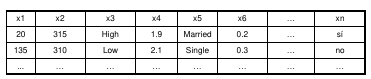
\includegraphics[scale=.85]{images/mod01-18.png}
\end{center}
si hay alguna/s variable/s de salida y/o de entrada. Las \tb{variables de salida} representan lo que quiero \tb{predecir} a partir de las \tb{variables de entrada}. En el caso que tenemos, $X_n$ es una \ti{variable de salida}, y el resto de variables, $X_1,X_2,\ldots$, serían \ti{variables de entrada}. En el momento en que determinamos la existencia de una/s variable/s de salida, hemos establecido una \tb{tarea predictiva}.

Por ejemplo, quiero saber si a un cliente hay que darle un préstamo, o una operación con tarjeta de crédito es fraudulenta o las ventas del próximo trimestre, etc. Todas son tareas que tienen un valor de salida a partir de valores de entrada.

Podemos distinguir dos tipos de \ti{tareas predictivas}:
\begin{itemize}
    \item \tb{Clasificación/Categorización}. Tenemos una \ti{variable de salida}, el resto son \ti{variables de entrada}, el valor de la variable predictiva es \tb{nominal} o \tb{cualitativa}. Por ejemplo, predecir si se concederá un crédito da como resultado una variable cualitativa o nominal, \tb{sí o no}, hablamos de una \ti{tarea de clasificación}.
    \item \tb{Regresión}. Si la \ti{variable de salida} es numérica. Por ejemplo, cuando queremos saber cuantos productos puedo vender en el trimestre.
\end{itemize}

Pero y cuando no hay ninguna \tb{variable de salida}, hablariamos de una \tb{tarea descriptiva}, muchas de las tareas del \ti{aprendizaje automático} son descriptivas, no predicen nada. Hay tareas \ti{descriptivas} que tienen un valor a la hora de entender y extraer conocimiento a partir de los datos. Por ejemplo, si lo que quiero hacer es entender las filas o las columnas, tengo diferentes tareas descriptivas.

Los tipos de \ti{tareas descriptivas} son.
\begin{itemize}
    \item \tb{Clustering}, si quiero entender la relación entre las filas de la tabla, relación entre individuos en este caso, si éstos fueran clientes puedo hacer un \ti{agrupamiento de clientes}, \ti{clustering de clientes}. Es una tarea cuyo objetivo es describir grupos de datos, que grupos de clientes tengo.
    \item \tb{Análisis Exploratorio}, es el análsis de las relaciones entre columnas:
    \begin{itemize}
        \item \tb{Reglas de asociación, dependencias funcionales}, cuando las variables son \tb{nominales, cualitativas}, no son números. Por ejemplo, las columnas que hacen referencia a \ti{alto, bajo, casado, soltero,\ldots} son nominales. Si el valor de \ti{High} en la variable $X_3$ está asociado con un valor de \ti{Married} en la variable $X_5$, sólo podré verlo si hay muchísimos ejemplos, ver si esta relación es más frecuente que otras. Otro ejemplo sería el \ti{análisis de la compra}, ver que productos se compran conjuntamente, ejemplo típico de las \tb{reglas de asociación}.
        \item \tb{Análsis Factorial o Multivariante}, si las variables que queremos relacionar son numéricas. El concepto de \ti{relación binaria}, cuando hablamos de este tipo de variables, se conoce tradicionalmente como \tb{correlación}. Entre las variables $X_4$ y $X_6$ podría ver si estos valores están correlacionados, por ejemplo, si la edad y el sueldo están correlacionados. Es un ámbito inmenso, que restringimos normalmente a preguntas más básicas como calcular correlaciones y una matriz de correlaciones. Esta última clasificación, también la conocecmos como \tb{análisis factorial de correlaciones, análisis de dispersión o análsis multivariable}.
    \end{itemize}
\end{itemize}

La pregunta es ¿qué ocurre si tengo varias variables numéricas y varias nominales?.
\begin{itemize}
    \item Si tenemos \ti{muchas numéricas y pocas nominales}, podemos \ti{numerizar todas las variables} y realizar un \tb{análisis de correlaciones}.
    \item Si tenemos \ti{muchas nominales y pocas numéricas}, las numéricas podemos \tb{discretizarlas} y realizar un \tb{análisis de regla de asociación}.
\end{itemize}

Son tipos de variables que no podemos analizar al mismo tiempo, pero podemos convertir unas en otras y aplicar el análisis que más convenga.

Es una manera simple, pero elegante de entender qué tipos de \tb{tareas} podemos tener en \ti{aprendizaje automático}, las difrencias fundamentales son:
\begin{itemize}
    \item \tb{predictivas}, qué tipo de variable tenemos que predecir, numérica o nominal.
    \item \tb{descriptivas}, queremos analizar las relaciones entre filas, \ti{agrupamientos}, o analizar relaciones entre columnas, \ti{análisis exploratorio}, si los valores son numéricos, \ti{correlaciones}, si son nominales, \ti{asociaciones}.
\end{itemize} 

¿Qué tipo de tare es \ti{«diagnostiscar la presencia de una enfermedad dados unos síntomas»}?:

\begin{enumerate}[label=\Alph*)]
    \item Clasificación
    \item Regresión 
    \item Asociación
    \item Clustering
\end{enumerate}

\tb{Solución: \ti{A)}, clasificación}.

\subsection{Técnicas}

En un ámbito general, las tareas de minería de datos o en ciencia de datos (aprendizaje automático), se dividían en cinco clases principales, dependiendo de si eran:
\begin{itemize}
    \item \tb{supervisadas}, 
    \item \tb{no supervisadas}, 
    \item \tb{predictivas} o 
    \item \tb{no predictivas}
\end{itemize} 

Es habitual confundir \ti{tareas} con \ti{técnicas} ya que muchas o algunas de las técnicas sólo resuelven un subconjunto o incluso una sóla de las tareas que hemos visto.

La tabla simplifica la relación entre \ti{tareas}

\begin{center}
    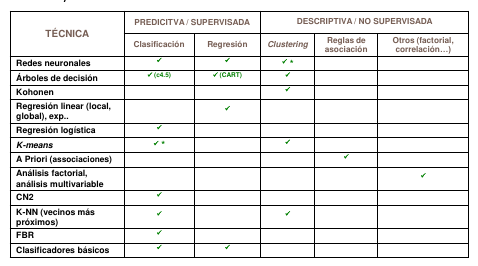
\includegraphics[scale=.6]{images/mod01-19.png}
\end{center}

La diferencia entre trea y técnica es importante ya que si no confundiremos el problema que queremos resolver.

Veamos de forma descriptiva alguna de estas técnicas:

\begin{itemize}
    \item \tb{Técnicas descriptivas}:
    \begin{itemize}
        \item \tb{Correlaciones y Asociaciones}, se suele denominar como \ti{análisis exploratorio}, y aquí tenemos:
        \begin{itemize}
            \item \tb{Coeficiente de correlación}, cuando hablamos de variables numéricas y matrices de correlación, y queremos analizar más de dos variables. En principio el coeficiente de correlación es \tb{bivariante}, ya que analizaría dos variables.
            \item \tb{Asociaciones}, hablamos de relaciones entre variables cualitativas, no numéricas, o categóricas. El ejemplo típico es la cesta de la compra, podemos preguntarnos si tabaco y alcohol están o no relacionados cuando se compran conjuntamente.
            \item \tb{Dependencias funcionales}, queremos conocer si una variable implica normalmente los valores de otra, se trata de una versión generalizada de las \ti{reglas de asociación}.
        \end{itemize}
        \item \tb{Clustering}, normalmente se dividen en:
        \begin{itemize}
            \item \tb{Jerárquicos}, tenemos lo que se denomina un \tb{dendograma}, en el que se agrupan ejemplos.
            \begin{center}
                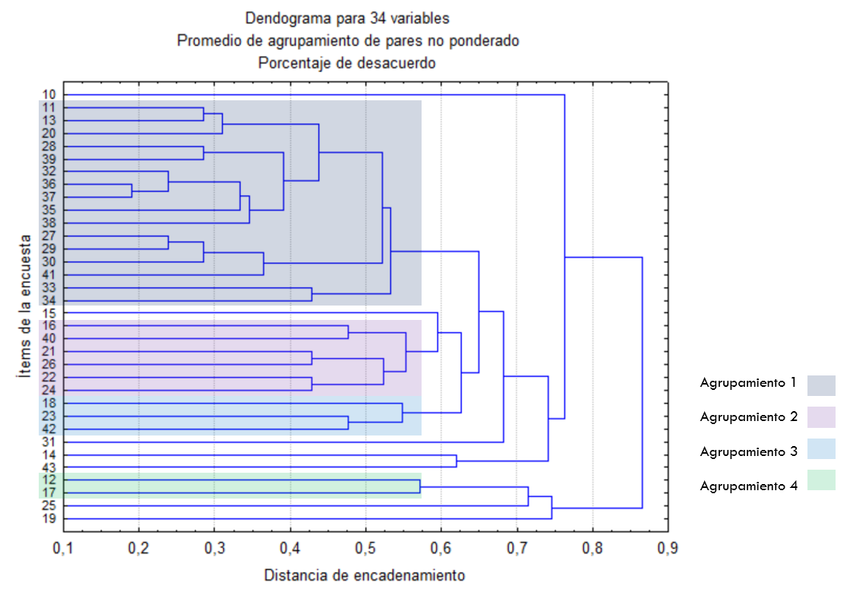
\includegraphics[scale=.4]{images/mod01-20.png}
            \end{center}
            Son ejemplos que se agrupan por distancia de enlazado, al final podemos partir en los grupos que deseemos.
            \item \tb{No Jerárquicos}, agrupan directamente en tres o cuatro grupos sin crear una jerarquía.
        \end{itemize}
        \item kkkk
    \end{itemize}
    \item \tb{Técnicas predictivas}. Se refiere a los tipos de \ti{regresión}:
    \begin{itemize}
        \item \tb{Regresión lineal}, problemas de regresión, con variables de salida cuantitativa y numérica.
        \item \tb{Regresión logística}, adaptación de la regresión lineal para problemas de clasificación, la variable de salida es \ti{cualitativa}.
        \item \tb{Regresión no lineal}, permite adaptarse a patrones, que de inicio, no son lineales.
    \end{itemize}

    \begin{center}
        \begin{tabular}{ c c }
            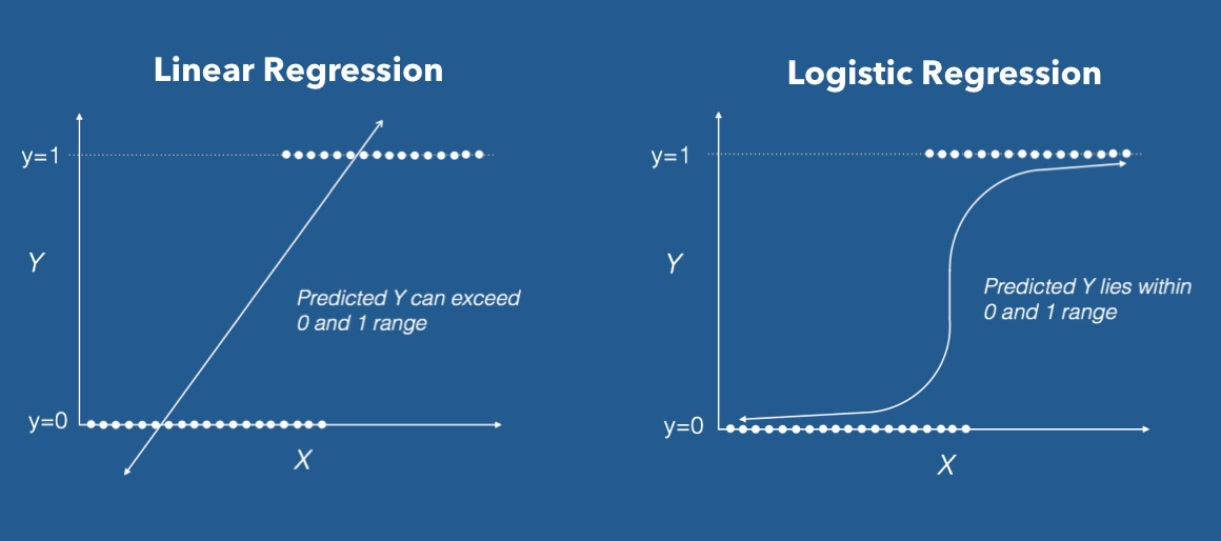
\includegraphics[scale=.65]{images/mod01-21_1.jpg} &
            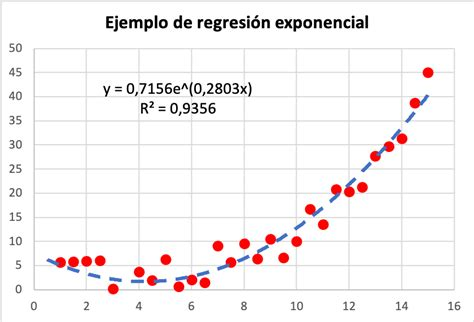
\includegraphics[scale=.35]{images/mod01-21_2.jpg}    
        \end{tabular}
    \end{center}
    Suelen verse juntas porque están muy relacionadas.
\end{itemize}

Veamos brevemente una serie de técnicas, una bastante antigua y usual es la denominada \ti{vecinos más próximos}, muy intuitiva, se categoriza o predice dependiendo de sus vecinos; para determinar los vecinos hay una distancia, una medida de similitud y, a través de ella, se miden cuáles son los vecinos más próximos a un nuevo ejemplo. De ese nuevo ejemplo no tenemos la categoría, la clase. Lo que se hace es mirar cuáles son los vecinos más próximos y a partir de ahí determinar de qué clase es.

\begin{center}
    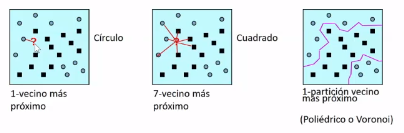
\includegraphics[scale=.9]{images/mod01-22.png}
\end{center}

Si hablamos del vecino más próximo, sólo se mira uno, es menos robusto porque puede haber \ti{«ruido»}, puede ser que un grupo pueda estar rodeado de cuadraditos y el vecino más cercano pueda ser un círculo, cerca del punto que quiera predecir. La partición que se hace es muy parecida a la que hariamos con un lápiz si intentaramos determinar fronteras entre las clases, en la imagen entre cuadrados negros y círculos verdes.

Otro ejemplo bastante popular son las \ti{redes neuronales}, y lo son por las aplicación de las \ti{redes neuronales profundas} (las \ti{redes neuronales no profundas} son sólo una capa oculta), se utilizan para muchas tareas, especialmente en las que las variables de entrada son bastante predictivas y no hay que crear nuevas características a partir de los datos. 

\begin{center}
    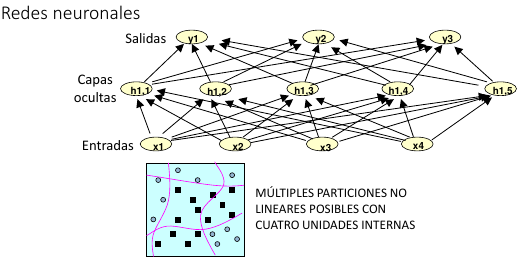
\includegraphics[scale=.9]{images/mod01-23.png}
\end{center}

La ventaja que tienen las \ti{redes neuronales}, de una capa o múltiples capas ocultas, es que permiten comportamientos \tb{no lineales} como el mostrado en la imagen. Las fronteras se combinan a través de lineas que no son lineales, pudiendo ajustarnos a las formas que producen los datos como nosotros queramos.

Los \ti{árboles de decisión} son muy comunes y es otra forma sencilla de entender los modelos extraídos utilizan técnicas que pueden representarse como un árbol, y se pueden representar en forma de reglas. Es una técnica muy utilizada en los entornos donde prima la \ti{comprensibilidad}.

\begin{center}
    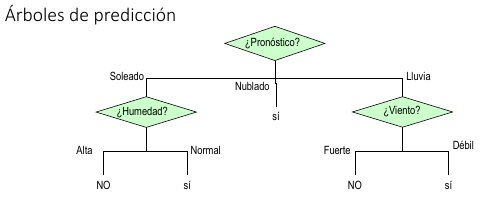
\includegraphics[scale=.95]{images/mod01-24.png}
\end{center}

A partir de los datos generamos un modelo, que dependiendo de tres variables: pronóstico, humedad y viento, podría determinar cuál será la clase de salida mediante los valores.
\begin{itemize}
    \item Si pronóstico soleado, 
    \item Si pronóstico nublado,
    \item Si pronóstico lluvia,
    \item Si viento fuerte,
    \item Si viento débil,
    \item Si humedad alta,
    \item Si humedad baja
\end{itemize}

Para tomar una decisión particular no tengo que evaluar todas las variables.

De la siguiente lista señaal las \tb{tareas}:

\begin{enumerate}[label=\Alph*)]
    \item Regresión lineal
    \item Clasificación 
    \item Regresión
    \item Custering (agrupamiento)
    \item Redes neuronales 
    \item Correlaciones 
    \item Regresión Logística 
    \item Reglas de asociación
    \item Vecinos más próximos
\end{enumerate}

\tb{Solución}: \ti{B), C), D), F) y H)}

\subsection{Herramientas}

Para llevar a cabo las técnicas que hemos visto, y muchas más, se recurre a herramientas, en las que normalmente ya están implementadas dichas técnicas, ya sea en forma visual o mediante lenguajes de programación mediante el uso de librerías, o con programación orientada a objetos y librerías específicas como ocurre con \ti{Python} o \ti{R}.
\begin{center}
    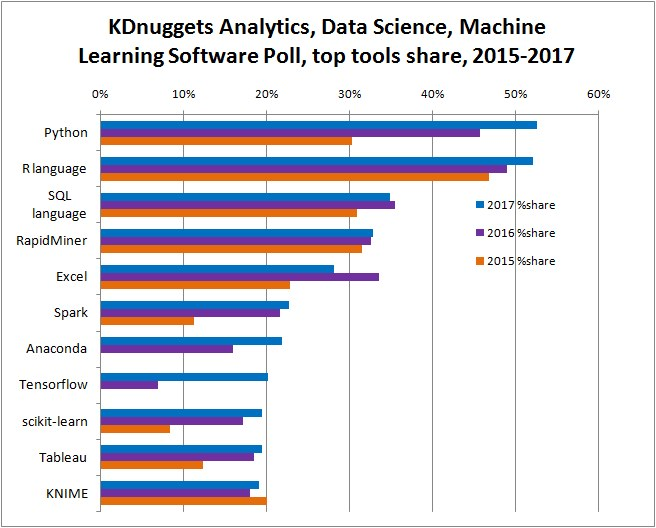
\includegraphics[scale=.45]{images/mod01-25.jpg}
\end{center}
Muchas de estas herramientas son gratuitas.

Lo interesante es ver que algunas de las herramientas se utilizan bastante en la comunidad:
\begin{itemize}
    \item \ti{R} y \ti{Python} son muy utilizadas y además son gratuitas.
    \begin{itemize}
        \item \tb{R}, es un lenguaje interpretado, que dispone de muchas librerías, pero es necesario saber programar, crear código, lo que tiene ventajas y desventajas. Una de las grandes ventajas que tiene es que dispone de librerías de visualización muy potentes, por ejemplo \tb{ggplot}.
        \item \tb{Python}, ha ido tomando espacio a \ti{R} como lenguaje de programación predominante en el análisis de datos, especialmente a partir de aparecer la librería \tb{Scikit-learn}, ésta contiene gran cantidad de técnicas de aprendizaje automático (\ti{R} también dispone de algunas librerías de este tipo).
    \end{itemize}
    \item Existen otro tipo de herramientas, estilo \ti{RapidMiner}, que son más visuales, más sencillas de manejar, pero que suelen tener una licencia que ya no es completamente abierta.
    \item Están las herramientas comerciales, cuyo uso requiere de la compra de licencias, están relacionadas con el \ti{BigData} y no tanto con el \ti{aprendizaje automático}.
    \item Existe una serie de herramientas adicionales que podemos utilizar en muchos casos, que aunque no sean propiamente de análisis de datos o de aprendizaje automático son muy utilizadas; es el caso de \ti{SQL}, muy utilizado cuando se trabaja con bases de datos, pero no es una herramienta de análisis, por el momento.
\end{itemize}. 

En la «nube» hay plataformas que permiten hacer el \ti{aprendizaje automático} como son: AzureML y BigML, pero hay muchas otras.

Existen otras muchas herramientas que se \ti{pagan por cómputo}, como \tb{TensorFlow}, que podemos instalar en nuestra máquina pero si requiere hacer redes profundas y tienes unos clusters, en principio, a veces, es más cómodo lanzar todo esto mediante algún \ti{servicio en la nube}, lo mismo ocurre con \ti{Keras}. Todas estas herramientas, más sofisticadas, suelen utilizar en \ti{aprendizaje profundo, reconocimiento de imágenes o de lenguaje natural}.